\documentclass{article}
\usepackage{graphicx}
\graphicspath{ {../images/} }
\usepackage{float}
\title{CS433 Assignment 2}
\author{Shaik Awez Mehtab (23b1080)
        \\ Evuri Mohana Sreedhara Reddy (23b1017)}
\date{}
\begin{document}
    \maketitle
    Here we present the plots we have generated and our understanding of why
    they were so:
    \section*{\texttt{restartmargin}}
    \begin{figure}[H]
        \centering
        \begin{minipage}{0.45\textwidth}
            \centering
            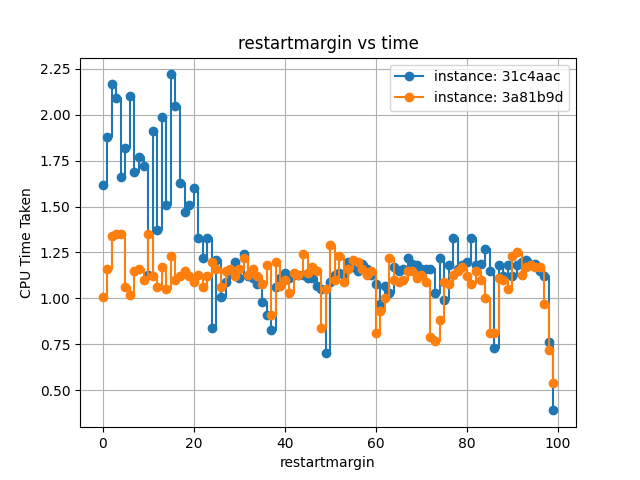
\includegraphics[width = \linewidth]{restartmargin-0.png}
        \end{minipage}
        \hfill
        \begin{minipage}{0.45\textwidth}
            \centering
            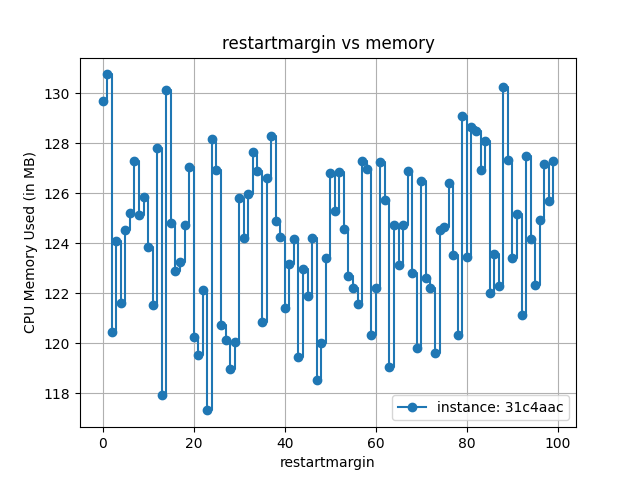
\includegraphics[width = \linewidth]{restartmargin-1.png}
        \end{minipage}
    \end{figure}
    As we can see from these figures there are sudden \textbf{drops} in time
    taken at few discrete values of \texttt{restartmargin}. This parameter
    relates with the frequency of restarts. This is done using something known
    as \textbf{glucose level}. Glucose level of a learned clause is based on
    how many of its literals appear in recent conflicts. Thus a newly learned
    clause which is getting involved in multiple conflicts has a high glucose
    level. If the average glucose level gets more than initial glucose
    * \texttt{restartmargin}, then there's a restart. This can be seen in
    \texttt{src/restart.cpp}. Small changes in this don't change timing much.
    But at certain threshold valuees as seen here, restart frequency aligns
    optimally with the problem structure, allowing solver to escape inefficient
    search regions at the right moment.

    \section*{\texttt{restartint}}
    \begin{figure}[H]
        \centering
        \begin{minipage}{0.45\textwidth}
            \centering
            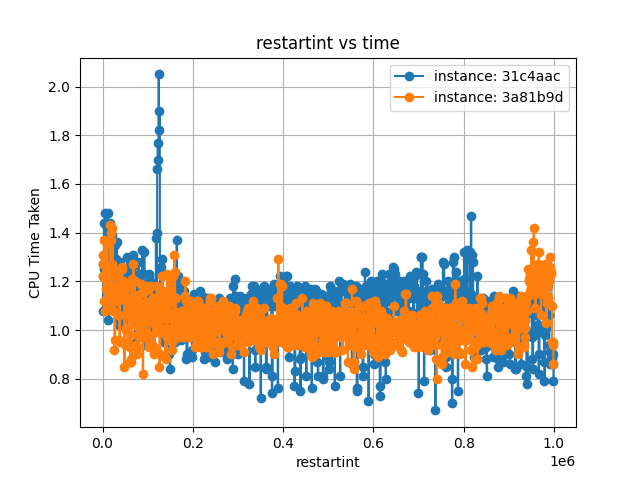
\includegraphics[width = \linewidth]{restartint-0.png}
        \end{minipage}
        \hfill
        \begin{minipage}{0.45\textwidth}
            \centering
            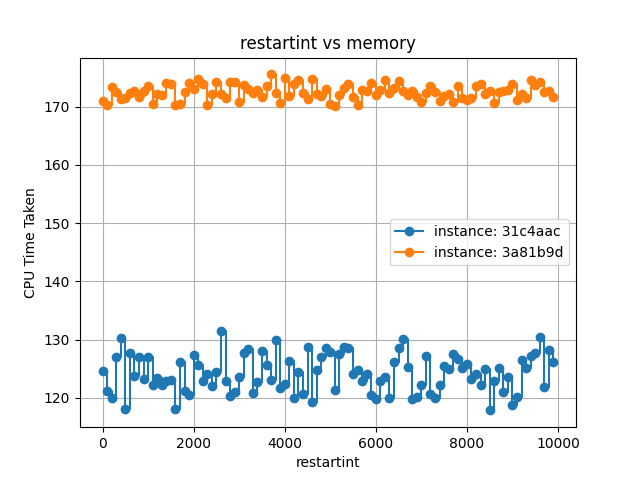
\includegraphics[width = \linewidth]{restartint-1.png}
        \end{minipage}
    \end{figure}

    As we can see from the figures, with an increase in \texttt{restartint},
    the time taken is expected to initially decrease, but after a certain
    point, it may start to increase again. \texttt{restartint} controls the
    interval between restarts, and increasing it delays restarts, allowing the
    solver to explore the search space more deeply before resetting. This can
    be beneficial by reducing unnecessary restarts and improving the solver’s
    progress with learned clauses. However, if the interval becomes too long,
    the solver might get stuck in unproductive areas of the search space,
    leading to longer solving times. So, while increasing \texttt{restartint}
    generally improves performance, there’s a balance, and beyond a certain
    threshold, it might have diminishing returns or even negative effects

    \section*{\texttt{reluctant}}
    \begin{figure}[H]
        \centering
        \begin{minipage}{0.45\textwidth}
            \centering
            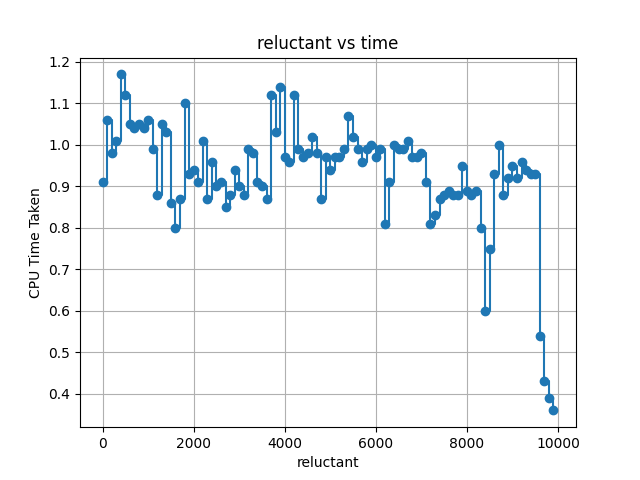
\includegraphics[width = \linewidth]{reluctant-0.png}
        \end{minipage}
        \hfill
        \begin{minipage}{0.45\textwidth}
            \centering
            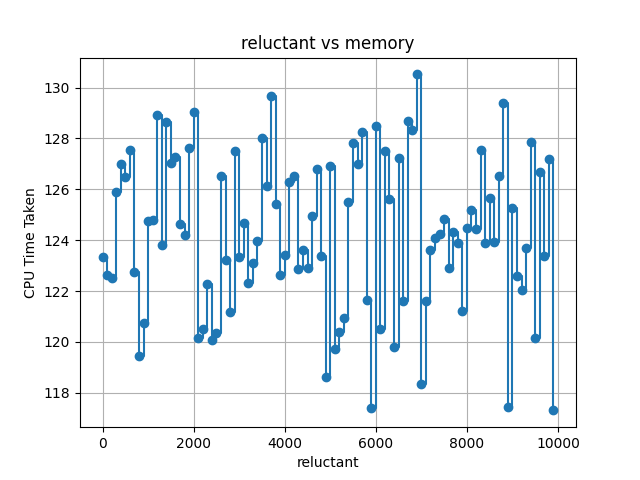
\includegraphics[width = \linewidth]{reluctant-1.png}
        \end{minipage}
    \end{figure}

    As we can see from the figures, with an increase in \texttt{reluctant},
    the time taken decreases. This might be because a higher \texttt{reluctant}
    causes the solver to delay restarts for a longer period, allowing it to
    explore the search space more deeply before resetting. By doing so, it can
    often make better decisions based on the learned clauses, avoiding
    unnecessary backtracking. As a result, the solver can find solutions more
    efficiently, reducing the overall time. This behavior is particularly
    noticeable when the solver benefits from not restarting too soon and is
    able to capitalize on previously learned information to make progress.

    \section*{\texttt{reluctantmax}}
    \begin{figure}[H]
        \centering
        \begin{minipage}{0.45\textwidth}
            \centering
            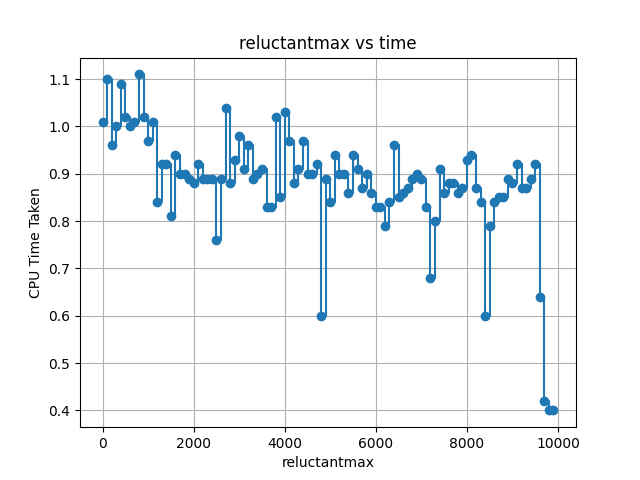
\includegraphics[width = \linewidth]{reluctantmax-0.png}
        \end{minipage}
        \hfill
        \begin{minipage}{0.45\textwidth}
            \centering
            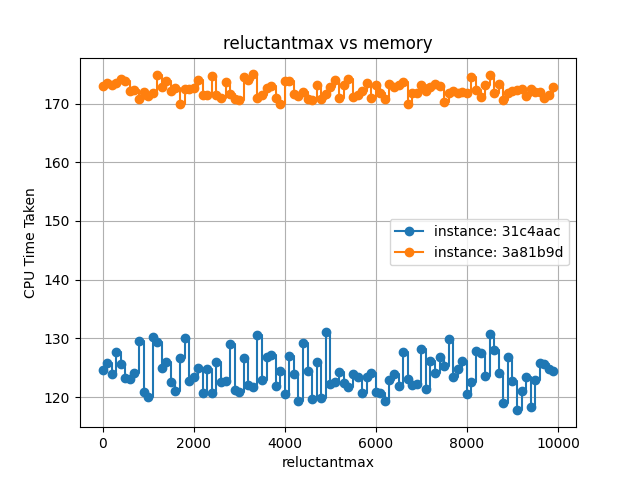
\includegraphics[width = \linewidth]{reluctantmax-1.png}
        \end{minipage}
    \end{figure}
    As we can see from these figures, there are sudden \textbf{drops} in time
    taken at a few discrete values of \texttt{reluctantmax}. This parameter
    controls the solver’s \textbf{reluctant doubling} restart strategy, where
    restart intervals grow progressively longer. Unlike \texttt{restartmargin},
    which reacts to glucose levels, this method follows a structured sequence
    based on an internal counter. The implementation can be found in
    \texttt{src/restart.cpp}.

    The sudden drops occur because \texttt{reluctantmax} defines restart timing
    in a \textbf{discrete, exponential manner}. At most values, changes in
    \texttt{reluctantmax} do not significantly affect when restarts happen,
    keeping the solving time stable. However, at certain points, the adjusted
    restart schedule aligns better with conflict patterns, allowing the solver
    to escape inefficient search paths earlier, leading to a sharp decrease in
    time taken.

    \section*{\texttt{restart}}
    \begin{figure}[H]
        \centering
        \begin{minipage}{\textwidth}
            \centering
            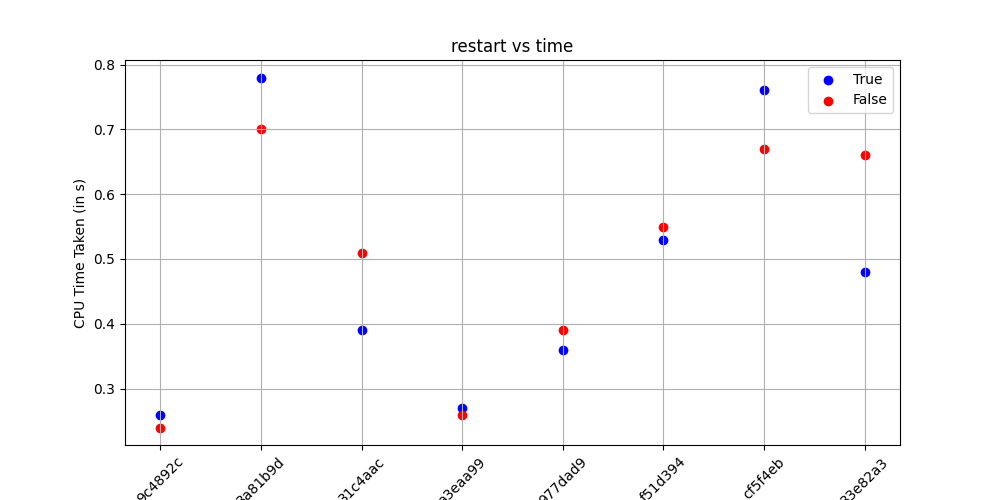
\includegraphics[width = \linewidth]{restart-0.png}
        \end{minipage}
        \hfill
        \begin{minipage}{\textwidth}
            \centering
            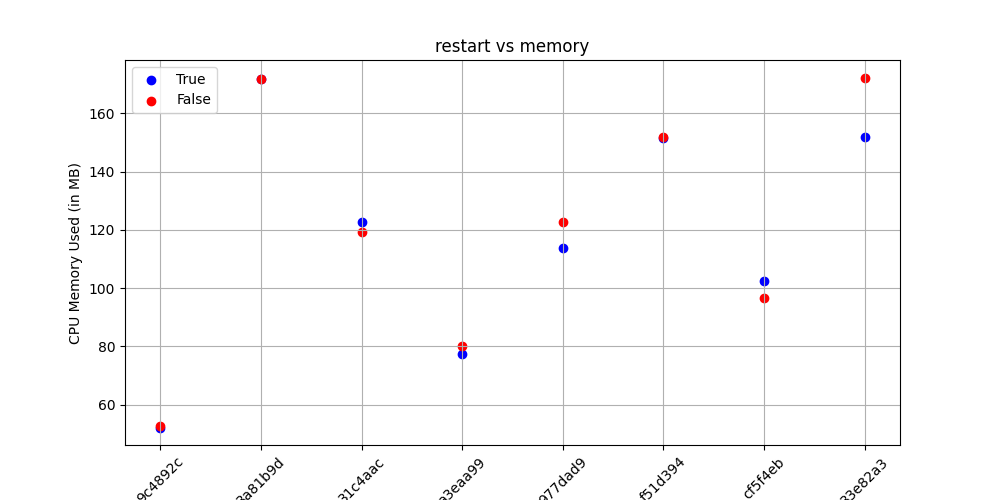
\includegraphics[width = \linewidth]{restart-1.png}
        \end{minipage}
    \end{figure}
    From the results, we can see that keeping \texttt{restart} = True is
    sometimes better, sometimes worse, and in some cases, nearly the same as
    False. This might be happening because the impact of restarts depends on
    the problem structure. When restarts help escape difficult search regions,
    they improve performance, but if they occur too frequently, they might
    disrupt useful clause learning, leading to slower solving. In cases where
    the search space is naturally well-guided, restarts make little difference,
    resulting in similar solving times. This explains why the trend varies
    instead of showing a clear preference.

    \section*{\texttt{restartreusetrail}}
    \begin{figure}[H]
        \centering
        \begin{minipage}{\textwidth}
            \centering
            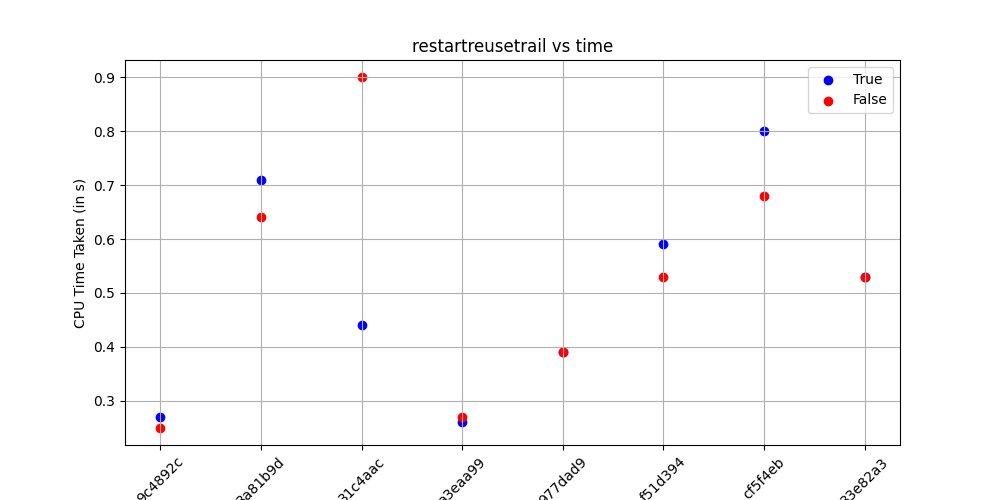
\includegraphics[width = \linewidth]{restartreusetrail-0.png}
        \end{minipage}
        \hfill
        \begin{minipage}{\textwidth}
            \centering
            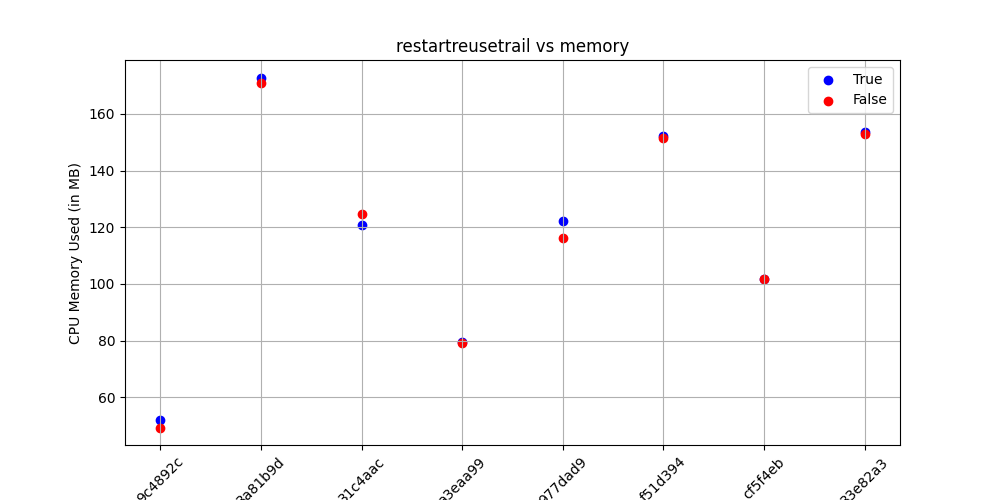
\includegraphics[width = \linewidth]{restartreusetrail-1.png}
        \end{minipage}
    \end{figure}
    From the results, setting \texttt{restartreusetrail} = True is just as
    often better as it is worse compared to False. This happens because reusing
    the trail after a restart can sometimes preserve useful decisions, making
    solving faster, but other times it keeps bad assignments, leading to more
    conflicts. If the problem benefits from continuity, it helps, but if a
    clean slate is better, it hurts. Since this entirely depends on the
    problem, neither setting is consistently the best.

\end{document}
